\chapter{Random test}\noindent
In this chapter, we investigate how LaTeX renders random mathematical expressions and cross-references and citations and stuff that we throw at it.
The chapter starts with a test of mathematical expressions in \cref{sec:test}, and continues with a \emph{Lorem Ipsum} citation in \cref{sec:test2}, and has miscellaneous footnotes inbetween.



\section{Here be random text about \textsc{srt/lrt}}\label{sec:test}
\textit{This is a Rapid Jabby Quaint Poem Kalif test.}\\
Written by \textsc{jabir ali ouassou}.
Roman number II IV or \textsc{ii} \textsc{iv} and Ⅲ and \textsc{Ⅲ}.
Let's see how this goes! Btw, $e^{i\pi} = -1$ and $(\partial_\mu \partial^\mu - m^2) \psi = 0$.
Also calligraphic $\mathcal{A} = \mathcal{F}x$.
Bold $\symbf{A}\symbf{\xi} = \symbf{\Delta}\symbf{\eta}$ and spins $\nabla^2 f_{\uparrow\downarrow}^{\vphantom{\dagger}}+\hat{\symbf{f}}_t\check{\symbf{g}}_s\hat{g}_{\downarrow\uparrow}^{\vphantom{\dagger}} - h_\perp^{\vphantom{*}} \times v_\parallel^{\vphantom{*}}.$
Some not-really-blackboard fonts $n \in \mathbb{N}_+$, $q \in \mathbb{Z}_2$, $r \in \mathbb{R}\,\backslash\,\{0\}$, $z \in \mathbb{C}$, $s \in \mathbb{S}$. 
Also $\partial_z I \sim \partial_z \Delta = 0$ and $\symbf{g}_{\up\dn} = \langle \{ \Psi^\dagger_\sigma(x) c^\ast_\dn(\symbf{r},t) \} \rangle$.
Also, we know well that $I(\phi) = I_0 \sin(\phi) + I_1' \sin(\delta\phi/2)$\footnote{This is simply just a simple test, with an equation $\sin a = \cos(2b-1)/\cos(2b+1)$. And here is a chemical element \ce{CrO23} and physical unit \SI{12e3}{m}. }.
\begin{equation}
  \nabla\cdot \symbf{E} = \langle \{ \Psi^\dagger_{\sigma\sigma'}(x) c^\ast_{\dn\up}(\symbf{r},t) \} \rangle.
\end{equation}
\begin{equation}
  \hat{g}^{\textsc{R}\dagger}_{\up\dn}\hat{h} - \hat{h}\hat{g}^{\textsc{k}} = \sigma_2(g_{\symup{s}} \sigma_0 + \symbf{g}_{\hspace{0.05em}\symup{t}}\cdot\symbf{\sigma})\sigma_2
\end{equation}
\begin{equation}
  \check{g} = \begin{pmatrix} \hat{g}^{\textsc{r}} & \hat{g}^{\textsc{k}} \\ 0^{\phantom{k}} & \hat{g}^{\textsc{a}} \end{pmatrix}
\end{equation}
\begin{equation}
  \hat{g}^{\textsc{r}} = \begin{pmatrix} \phantom{-}g\; & \phantom{-}f\;\; \\ -\tilde{f}\; & -\tilde{g}\;\; \end{pmatrix}
= \begin{pmatrix} \phantom{-}N(1+\gamma\tilde{\gamma}) & \phantom{-}2N\gamma\;\; \\ -\tilde{N}(1+\tilde{\gamma}\gamma) & -2\tilde{N}\tilde\gamma\;\; \end{pmatrix} 
\end{equation}
\begin{equation}
  \Delta(z) = \int_0^{\infty} \mathrm{d}\epsilon\,\mathrm{Re}\big[f_{\symup{s}}(\epsilon)\big] \tanh\!\left(\frac{\symup\pi}{2e^{\symup{\gamma}}} \frac{\epsilon/\Delta_0}{T/T_{\symup{c}}}\right)
\end{equation}
Alternatively without any \textsc{iso} standards complicance (i.e. multiletter as only criterion for upright):
\begin{equation}
  \Delta(z) = \int_0^{\infty} \mathop{d\kern-0.02em\epsilon}\mathrm{Re}\big[f_s(\epsilon)\big] \tanh\!\left(\frac{\pi}{2e^{\gamma}} \frac{\epsilon/\Delta_0}{T/T_{c}}\right)
\end{equation}
Testing super and subscripts:
\begin{equation}
  \nabla \cdot \symbf{I}_{i} = \symbf{Q}_{ij} h_j + M_{ij} \nabla h_j, \quad 
  h_n = \frac{1}{4} \sum_n \mathrm{Tr}[\hat{h}\hat{\rho}_n].
\end{equation}
Some references are given in \cref{ch:test}, and more specifically \cref{sec:test,sec:test2}.
\begin{equation}
  \int \mathrm{d}x\, f(x) \sum_i n_i^\beta \prod_j p_j^\alpha
\end{equation}
Here is some normal text. \textit{And here is some emphasized text 1234567890}. Normal 123456789. 
Say something about the \textsc{bcs} theory and \textsc{bcs-bec} transition \emph{and \textsc{srt/lrt} in italics}.
This is another test: $1 < 2 > 0 \leq 1 \geq 2$, and here is an url: \url{http://www.google.com/interesting_something/else/and/even/more/stuff}
%\verb+for i=[0:0.1:1.0] do f(i,j) = 1/g(j,i)+
\begin{equation}
  \textit{e}e\mathrm{e}\textsf{e}\;%\texttt{e}\;
  \textit{I}I\mathrm{I}\textsf{I}\;%\texttt{I}\;
  \textit{m}m\mathrm{m}\textsf{m}\;%\texttt{m}
\end{equation}
Here is another one:
\begin{equation}
  a\alpha b\beta d\delta e\epsilon \chi\psi bd \phi\theta v\nu u p\rho \Gamma[P(\Psi)]
\end{equation}
\begin{align}
  \text{ABCDEFGHIJKLMOPQRSTUVWXYZ}~\text{Rough Kalɡ Just}\\
  ABCDEFGHIJKLMOPQRSTUVWXYZ\\
  abcdefghijklmopqrstuvwxyz
\end{align}
\textsf{And here is some sans-serif text with math $e^{i\phi}=\cos\phi+i\sin\phi$ and so on etc.} And here is some normal text again.
Here is a chemical equation \ce{CrO23} and unit \SI{23e23}{m/s} but $J_0 = \SI{23e23}{m/s}$ also.

Selfconsistency equation:
\begin{equation}
  \Delta_{n+1}(\symbf{r}) = F[\Delta_n(\symbf{r})]
\end{equation}

\section{Quasiclassical theory and Green's functions}\label{sec:test2}
Quasiclassical theory has been successful.
\textsc{quasiclassical theory} with regards to \textsc{bardeen--cooper-schrieffer (bcs)} theory.
Lorem ipsum dolor sit amet, consectetuer adipiscing elit.
Donec malesuada magna sem.
Fusce vitae lectus id magna convallis euismod.
Quisque viverra sollicitudin turpis, vel ultricies mauris dictum quis.
Praesent justo nunc, luctus in lectus in, placerat tempus orci.
\begin{equation}
  f(x) = \sin(x) + 1/\cos(x) + \mathrm{atan}(1/x)
\end{equation}
Donec placerat neque ac tortor dignissim pellentesque.
Aenean tellus erat, eleifend id interdum a, volutpat et massa.
Quisque tristique accumsan efficitur.

\begin{figure}[h!]
  \centering
  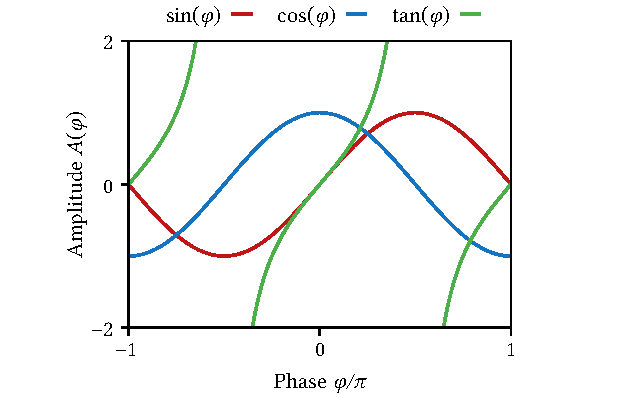
\includegraphics[width=0.2\textwidth]{test.jpg}
  \caption{This is simply a test figure, and equation $\sin(2x)=1$, and some \textsc{si} unit \SI{1.0e3}{m/s}, and some chemical \ce{CrO2}. This text can even be made even longer, since we want to test this properly.}
  \label{fig:test}
\end{figure}


Morbi non tortor volutpat, mattis odio at, tincidunt libero.
Donec pulvinar et mi at varius.
Sed vulputate lectus eu libero gravida, vel porta tortor bibendum.
Quisque dictum ex id quam ultrices, ut commodo nisl euismod.
Aliquam vulputate, urna quis sodales rhoncus, orci metus pulvinar velit, feugiat sollicitudin dui massa interdum tortor.
Nam sed ante vitae eros imperdiet bibendum.
Fusce pretium semper leo eget lobortis.
Sed dictum erat quis diam faucibus bibendum.
Integer vitae enim euismod, ornare augue quis, pharetra ante.
Phasellus venenatis tellus ut velit faucibus, posuere porttitor lacus hendrerit.

\begin{table}[h!]
  \centering
  \caption{This is simply a test table.}
  \label{tab:test}
  \begin{tabular*}{\dimexpr\textwidth-4em\relax}{@{\extracolsep{\stretch{1}}\,}lcc@{\,}}
    \toprule
    Name    &   Symbol    &   Value             \\
    \midrule
    Euler constant          & $e$   & $2.71...$  \\
    Circle constant         & $\pi$ & $3.14...$ \\
    Imaginary identity      & $i$ & $\sqrt{-1}$ \\
    \bottomrule
  \end{tabular*}
\end{table}

Lorem ipsum dolor sit amet, consectetur adipiscing elit.
Donec malesuada magna sem.
Fusce vitae lectus id magna convallis euismod.
Quisque viverra sollicitudin turpis, vel ultricies mauris dictum quis.
Praesent justo nunc, luctus in lectus in, placerat tempus orci.
Donec placerat neque ac tortor dignissim pellentesque.
Aenean tellus erat, eleifend id interdum a, volutpat et massa.
Quisque tristique accumsan efficitur.

Morbi non tortor volutpat, mattis odio at, tincidunt libero.
Donec pulvinar et mi at varius.
Sed vulputate lectus eu libero gravida, vel porta tortor bibendum.
Quisque dictum ex id quam ultrices, ut commodo nisl euismod.
Aliquam vulputate, urna quis sodales rhoncus, orci metus pulvinar velit, feugiat sollicitudin dui massa interdum tortor.
Nam sed ante vitae eros imperdiet bibendum.
Fusce pretium semper leo eget lobortis.
Sed dictum erat quis diam faucibus bibendum.
Integer vitae enim euismod, ornare augue quis, pharetra ante.
Phasellus venenatis tellus ut velit faucibus, posuere porttitor lacus hendrerit.

Lorem ipsum dolor sit amet, consectetur adipiscing elit.
Donec malesuada magna sem.
Fusce vitae lectus id magna convallis euismod.
Quisque viverra sollicitudin turpis, vel ultricies mauris dictum quis.
Praesent justo nunc, luctus in lectus in, placerat tempus orci.
Donec placerat neque ac tortor dignissim pellentesque.
Aenean tellus erat, eleifend id interdum a, volutpat et massa.
Quisque tristique accumsan efficitur.


\section{Continuation}
Morbi non tortor volutpat, mattis odio at, tincidunt libero.
Donec pulvinar et mi at varius.
Sed vulputate lectus eu libero gravida, vel porta tortor bibendum.
Quisque dictum ex id quam ultrices, ut commodo nisl euismod.
Aliquam vulputate, urna quis sodales rhoncus, orci metus pulvinar velit, feugiat sollicitudin dui massa interdum tortor.
Nam sed ante vitae eros imperdiet bibendum.
Fusce pretium semper leo eget lobortis.
Sed dictum erat quis diam faucibus bibendum.
Integer vitae enim euismod, ornare augue quis, pharetra ante.
Phasellus venenatis tellus ut velit faucibus, posuere porttitor lacus hendrerit.

Lorem ipsum dolor sit amet, consectetur adipiscing elit~\cite{feynman,statistics}\footnote{Testing footnotes}.
Donec malesuada magna sem.
Fusce vitae lectus id magna convallis euismod.
Quisque viverra sollicitudin turpis, vel ultricies mauris dictum quis.
Praesent justo nunc, luctus in lectus in, placerat tempus orci.
Donec placerat neque ac tortor dignissim pellentesque.
Aenean tellus erat, eleifend id interdum a, volutpat et massa.
Quisque tristique accumsan efficitur.

Morbi non tortor volutpat, mattis odio at, tincidunt libero.
Donec pulvinar et mi at varius.
Sed vulputate lectus eu libero gravida, vel porta tortor bibendum.
Quisque dictum ex id quam ultrices, ut commodo nisl euismod.
Aliquam vulputate, urna quis sodales rhoncus, orci metus pulvinar velit, feugiat sollicitudin dui massa interdum tortor\footnote{This is another footnote test.; This is simply just a simple test, with an equation $\sin \alpha = \cos(2a-1)/\cos(2a+1)$. And here is a chemical element \ce{CrO23} and physical unit \SI{12e3}{m}.; Here is another footnote, also set in sans-serif.}.
Nam sed ante vitae eros imperdiet bibendum. 
Fusce pretium semper leo eget lobortis.
Sed dictum erat quis diam faucibus bibendum.
Integer vitae enim euismod, ornare augue quis, pharetra ante.
Phasellus venenatis tellus ut velit faucibus, posuere porttitor lacus hendrerit.

Lorem ipsum dolor sit amet, consectetur adipiscing elit.
Donec malesuada magna sem.
Fusce vitae lectus id magna convallis euismod.
Quisque viverra sollicitudin turpis, vel ultricies mauris dictum quis.
Praesent justo nunc, luctus in lectus in, placerat tempus orci.
Donec placerat neque ac tortor dignissim pellentesque.
Aenean tellus erat, eleifend id interdum a, volutpat et massa.
Quisque tristique accumsan efficitur.

Morbi non tortor volutpat, mattis odio at, tincidunt libero.
Donec pulvinar et mi at varius.
Sed vulputate lectus eu libero gravida, vel porta tortor bibendum.
Quisque dictum ex id quam ultrices, ut commodo nisl euismod.
Aliquam vulputate, urna quis sodales rhoncus, orci metus pulvinar velit, feugiat sollicitudin dui massa interdum tortor.
Nam sed ante vitae eros imperdiet bibendum.
Fusce pretium semper leo eget lobortis.
Sed dictum erat quis diam faucibus bibendum~\cite{particle}\footnote{Test}.
Integer vitae enim euismod, ornare augue quis, pharetra ante.
Phasellus venenatis tellus ut velit faucibus, posuere porttitor lacus hendrerit.


\begin{align}
  \hat{g}^{\textsc{k}\ast}_{\up\dn}(\symbf{r},t) &= \big\langle\big[ \Psi^\dagger_{\up}(\symbf{r},t),\, \Psi_\dn^{\vphantom{\dagger}}(\symbf{r},t) \big]\big\rangle, \\
  \Delta^\ast_s &= \big\langle c^\dagger_{\up} c^{\vphantom{\dagger}}_{\dn} \big\rangle.\\
  e^{2\pi i n} = 1^n\\
  \symup{e}^{2\symup{\pi}\symup{i}θ} = 1+2\symup{i}\\
  1■2□3, \Delta = \Delta_0 e^{i\phi}, \Delta = \Delta_0e^{i\phi} \\
  f(x) \coloneq \sin(x) \phi\symup{i\pi\delta}(x) \symup{\delta}_{ij}
\end{align}
Perhaps using \textsc{iso} standard for standard functions is cumbersome...
Especially stuff like π-junction vs φ-junction, or $\symup{\pi}$-junction vs. $\phi$-junction is strange...
Most people don't know the up vs. slant notation, so even though it might clear up some index/imaginary and electron/euler ambiguities, it's a typographic nightmare for little gain.
Especially the distinction between standard math functions (like the deltas) and my own functions is weird.

\begin{align}
  \hat{\tau}_0 &= 
  \begin{pmatrix}
    +\sigma_0 & 0 \\
    0 & +\sigma_0
  \end{pmatrix}
  &
  \hat{\tau}_1 &= 
  \begin{pmatrix}
    0 & +\sigma_0 \\
    +\sigma_0 & 0 
  \end{pmatrix}
  &
  \hat{\tau}_2 &= 
  \begin{pmatrix}
    0 & -i\sigma_0 \\
    +i\sigma_0 & 0 
  \end{pmatrix}
  &
  \hat{\tau}_3 &= 
  \begin{pmatrix}
    +\sigma_0 & 0 \\
    0 & -\sigma_0
  \end{pmatrix}
  \\
  \hat{\sigma}_0 &=
  \begin{pmatrix}
    +\sigma_0 & 0 \\
    0 & +\sigma_0
  \end{pmatrix}
  &
  \hat{\sigma}_1 &=
  \begin{pmatrix}
    +\sigma_1 & 0 \\
    0 & +\sigma_1
  \end{pmatrix}
  &
  \hat{\sigma}_2 &=
  \begin{pmatrix}
    +\sigma_2 & 0 \\
    0 & -\sigma_2
  \end{pmatrix}
  &
  \hat{\sigma}_3 &=
  \begin{pmatrix}
    +\sigma_3 & 0 \\
    0 & +\sigma_3
  \end{pmatrix}
\end{align}

NOT Kronecker products because of cc.

\chapter{Lorem ipsum}\noindent
Lorem ipsum dolor sit amet, consectetur adipiscing elit.
Nullam vitae risus libero.
Nunc ut enim eget diam euismod mattis ac auctor sapien.
Sed sit amet dui condimentum, congue nisi non, dictum velit.
Suspendisse nec tortor id odio faucibus tempor eu in risus.
Quisque maximus lacus nisi, a ornare lectus convallis a.
Cras interdum rutrum sodales.
Curabitur a diam vestibulum, volutpat libero nec, bibendum odio.
Quisque vel ante in tortor imperdiet accumsan auctor sed nulla.
Aenean posuere felis massa, ac lacinia neque dictum sed.

\section{Here is a subsection}
Cras eu feugiat elit.
Cras ac turpis arcu.
Fusce in interdum risus, vel pharetra ante.
Orci varius natoque penatibus et magnis dis parturient montes, nascetur ridiculus mus.
Nulla ultrices hendrerit tincidunt.
Vivamus a luctus neque.
Praesent eu semper ligula, a ultricies dui.
Sed maximus, ante in mattis convallis, odio magna lobortis sapien, porta commodo turpis nunc id tortor.
Curabitur suscipit ipsum at arcu rhoncus molestie.
Quisque vestibulum, erat eget hendrerit interdum, est ipsum iaculis dui, eget rhoncus sapien libero quis est.
Nunc tristique ipsum tempus nulla aliquet, sit amet pharetra nibh venenatis.
Praesent non dignissim magna.
Integer euismod purus nulla, non rhoncus ligula hendrerit eu. Duis convallis a enim sit amet ultricies.
\begin{align}
  \nabla\cdot\symbf{D}  &= \rho, & 
  \nabla\times\symbf{E} &= 0 - \partial_{{\kern-0.075em}t{\kern0.04em}}\symbf{B};\\
  \nabla\cdot\symbf{B}  &= 0, &
  \nabla\times\symbf{H} &= \symbf{J} + \partial_{{\kern-0.075em}t{\kern0.04em}}\symbf{D}.
\end{align}

\begin{figure}[t!]
  \centering
  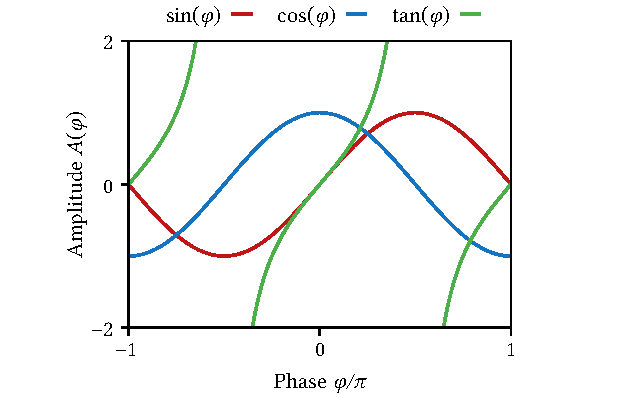
\includegraphics[width=\textwidth]{test.pdf}
  \caption
  {
    This is an example figure made by \textsc{gnuplot}. 
    I have also included an intentionally long caption to show the margins.
  }
\end{figure}

Etiam tristique sit amet massa nec finibus.
Pellentesque suscipit libero metus, vitae scelerisque urna commodo mattis.
Sed nec faucibus est, vulputate fringilla orci.
Fusce faucibus aliquet nulla.
Nam nec aliquet augue.
Maecenas eu augue luctus ipsum tincidunt malesuada quis eget enim.
Quisque in varius orci, ut eleifend eros.
Integer pulvinar euismod felis, eget placerat diam ultricies sit amet.
\[
  Q_{ij}\kern0.10em(\symbf{r},\symbf{r}'\kern-0.10em,t,t') = \sum_{nmk} A_{in}^\alpha(\symbf{r}) \, B_{nj}^\gamma(\symbf{r'}) \, [\Gamma(t-t')]^{2\pi\delta_k}
\]

Quisque varius commodo tellus, eget mollis urna auctor in.
Ut ut maximus turpis.
Aliquam erat volutpat.
Sed suscipit turpis massa, vel rutrum ipsum convallis in.
Aenean dignissim felis pharetra orci tempor dignissim ac eu lectus.
Mauris nec libero ante.
Phasellus nec finibus mi, vel mollis tortor.
Mauris diam est, venenatis sed tellus ut, maximus eleifend felis.
Fusce sollicitudin nec mauris non maximus.
Aenean massa lorem, euismod vel faucibus at, pretium eget ipsum.
Morbi sit amet maximus purus, et lacinia magna.
Pellentesque ex sem, rutrum et auctor quis, dignissim non massa.
Mauris congue libero vel lacus commodo facilisis.
Etiam faucibus at sapien in laoreet.
\begin{equation}
  \Delta(z) = \int_0^{\infty} \!\!\d\epsilon\, \re\!\big[f_s(\epsilon)\big] \tanh\!\left(\frac{\pi}{2e^{\gamma}} \frac{\epsilon/\Delta_0}{T/T_{\textrm{c}}}\right)
\end{equation}

Ut euismod augue tellus, eget eleifend lectus mollis sit amet.
Vestibulum ac erat leo.
Cras iaculis erat justo, at dignissim sem vehicula vitae.
Duis interdum odio vel lectus luctus pretium.
Phasellus molestie nec ex vitae semper.
Curabitur vel justo a libero blandit porttitor.
Cras aliquet erat non sem consectetur sodales.
Vivamus suscipit, metus in venenatis tincidunt, nibh nisl hendrerit libero, sit amet eleifend purus urna luctus erat.
Phasellus eu accumsan felis.
Integer imperdiet dolor at lectus feugiat, nec tristique nibh mollis.
Integer ac ligula et metus accumsan tristique. 

\lipsum
